%\documentclass[hyperref={pdfpagelabels=false},slidetop,9pt]{beamer}
\documentclass[slidetop,8pt]{beamer}
\usepackage[T1]{fontenc}
\usepackage[utf8]{inputenc}
\newcommand{\id}{54}
\newcommand{\nom}{Liaisons mécaniques}
\newcommand{\sequence}{04}
\newcommand{\num}{01}
\newcommand{\type}{TP}
\newcommand{\descrip}{Modélisation d'un solide. Comportement des liaisons mécaniques. Modéliser les mécanismes du laboratoire par un schéma cinématique, paramétré.}
\newcommand{\competences}{A3-C4: Analyse d'architecture et de comportement \\ &  Mod1-C1: Isolement d'un solide ou d'un système de solides \\ &  Mod2-C10-1: Modèle de solide indéformable \\ &  Mod2-C11: Modélisation géométrique et cinématique des mouvements entre solides indéformables \\ &  Mod2-C12: Modélisation cinématique des liaisons entre solides \\ &  Mod2-C15: Modélisation des actions mécaniques \\ &  Rés-C6: Utilisation d'un solveur ou d'un logiciel multi physique \\ &  Com1-C1: Différents descripteurs introduits dans le programme \\ &  Com2-C4: Outils de communication}
\newcommand{\nbcomp}{9}
\newcommand{\systemes}{Plateforme Stewart}
\newcommand{\systemessansaccent}{Plateforme Stewart}
\newcommand{\ilot}{2}
\newcommand{\ilotstr}{02}
\newcommand{\dossierilot}{\detokenize{Ilot_02 Plateforme Stewart}}
\newcommand{\imageun}{Plateforme}

\newcommand{\urlsysteme}{\href{https://www.costadoat.fr/systeme/57}{Ressources système}}
\newcommand{\matlabsimscape}{\href{https://github.com/Costadoat/Sciences-Ingenieur/raw/master/Systemes/Plateforme Stewart/Plateforme_Stewart_Simscape.zip}{Modèle Simscape}}
\newcommand{\solidworks}{\href{https://github.com/Costadoat/Sciences-Ingenieur/raw/master/Systemes/Plateforme Stewart/Plateforme_Stewart_Solidworks.zip}{Modèle Solidworks}}
\newcommand{\edrawings}{\href{https://github.com/Costadoat/Sciences-Ingenieur/raw/master/Systemes/Plateforme Stewart/Plateforme_Stewart.EASM}{Modèle eDrawings}}
\newcommand{\test}{Stewart_param1}
\newcommand{\testi}{Stewart_param2}
\newcommand{\testii}{Stewart_param3}
\newcommand{\testiii}{Stewart_param4}
\newcommand{\testiiii}{Stewart_euler}
\usepackage{etex}
\usepackage{tikz}
\usepackage[european]{circuitikz}
\usepackage{pgf}
\usepackage[all]{xy}
\usepackage{pgfpages}
\usepackage{graphbox}
\usepackage{pdfpages}
\usepackage[adobe-utopia]{mathdesign}
\usepackage{ifthen}
\usepackage{cancel}
\usepackage{framed}
\usepackage{subfig}
\usepackage{tabularx}
\usepackage{setspace}
\usepackage{soul}
\usepackage{schemabloc}
\usepackage{eqnarray}
\usepackage[dot, phantomtext]{dashundergaps}
\usepackage{media9}
\usepackage{multimedia}
\usepackage{textcomp}

\author{Renaud Costadoat}
\institute{Lycée Dorian}

\usepackage{multido}
\usepackage{multirow}
\usepackage{multicol} % Portions de texte en colonnes
\usepackage{flafter}%floatants après la référence

\usepackage{color}
\usepackage{xcolor}
\usepackage{colortbl}

\usepackage[gen]{eurosym}
\usepackage{tikz}
%\usepackage{pstricks,pst-node,pst-tree,pst-solides3d}
\usepackage{lmodern}
\usepackage[francais]{babel}
\usepackage{pslatex}
\usetheme{renaud}
\usepackage{times}
\usepackage{amsmath}
\usepackage{verbatim}
\usepackage{moreverb}
%\usetikzlibrary{arrows,shapes}
\usepackage{graphicx}
\usepackage{psfrag}
\usepackage{wrapfig}
\usepackage{etoolbox}

\definecolor{gris25}{gray}{0.75}
\definecolor{bleu}{RGB}{18,33,98}
\definecolor{bleuf}{RGB}{42,94,171}
\definecolor{bleuc}{RGB}{231,239,247}
\definecolor{rougef}{RGB}{185,18,27}
\definecolor{rougec}{RGB}{255,188,204}%255,230,231
\definecolor{vertf}{RGB}{103,126,82}
\definecolor{vertc}{RGB}{220,255,191}

\setlength\parindent{24pt}
\parskip 7.2pt
\parindent 8pt

\newenvironment{rem}[1][\hsize]%
{%
    \def\FrameCommand
   {%
\rotatebox{90}{\textit{\textsf{Remarque}}} 
       {\color{bleuf}\vrule width 3pt}%
       \hspace{0pt}%must no space.
       \fboxsep=\FrameSep\colorbox{bleuc}%
  }%
    \MakeFramed{\hsize#1\advance\hsize-\width\FrameRestore}%
}%
{\endMakeFramed}%


\newenvironment{savoir}[1][\hsize]%
{%
    \def\FrameCommand
    {%
\rotatebox{90}{\textit{\textsf{Savoir}}} 
        {\color{bleuf}\vrule width 3pt}%
        \hspace{0pt}%must no space.
        \fboxsep=\FrameSep\colorbox{bleuc}%
    }%
    \MakeFramed{\hsize#1\advance\hsize-\width\FrameRestore}%
}%
{\endMakeFramed}%

\newenvironment{prob}[1][\hsize]%
{%
    \def\FrameCommand%
    {%
\rotatebox{90}{\textit{\textsf{Problematique}}} 
        {\color{rougef}\vrule width 3pt}%
        \hspace{0pt}%must no space.
        \fboxsep=\FrameSep\colorbox{rougec}%
    }%
    \MakeFramed{\hsize#1\advance\hsize-\width\FrameRestore}%
}%
{\endMakeFramed}%

\newenvironment{obj}[1][\hsize]%
{%
    \def\FrameCommand%
    {%
\rotatebox{90}{\textit{\textsf{Objectif}}} 
        {\color{vertf}\vrule width 3pt}%
        \hspace{0pt}%must no space.
        \fboxsep=\FrameSep\colorbox{vertc}%
    }%
    \MakeFramed{\hsize#1\advance\hsize-\width\FrameRestore}%
}%
{\endMakeFramed}%

\newenvironment{defi}[1][\hsize]%
{%
    \def\FrameCommand%
    {%
\rotatebox{90}{\textit{\textsf{Definition}}} 
        {\color{bleuf}\vrule width 3pt}%
        \hspace{0pt}%must no space.
        \fboxsep=\FrameSep\colorbox{rougec}%
    }%
    \MakeFramed{\hsize#1\advance\hsize-\width\FrameRestore}%
}%
{\endMakeFramed}%


\newenvironment{hypo}[1][\hsize]%
{%
    \def\FrameCommand%
    {%
\rotatebox{90}{\textit{\textsf{Hypothèse\\}}} 
        {\color{bleuf}\vrule width 3pt}%
        \hspace{0pt}%must no space.
        \fboxsep=\FrameSep\colorbox{bleuc}%
    }%
    \MakeFramed{\hsize#1\advance\hsize-\width\FrameRestore}%
}%
{\endMakeFramed}%


\newenvironment{prop}[1][\hsize]%
{%
    \def\FrameCommand%
    {%
\rotatebox{90}{\textit{\textsf{Propriété}}} 
        {\color{bleuf}\vrule width 3pt}%
        \hspace{0pt}%must no space.
        \fboxsep=\FrameSep\colorbox{bleuc}%
    }%
    \MakeFramed{\hsize#1\advance\hsize-\width\FrameRestore}%
}%
{\endMakeFramed}%

\newenvironment{props}[1][\hsize]%
{%
    \def\FrameCommand%
    {%
\rotatebox{90}{\textit{\textsf{Propriétés}}} 
        {\color{bleuf}\vrule width 3pt}%
        \hspace{0pt}%must no space.
        \fboxsep=\FrameSep\colorbox{bleuc}%
    }%
    \MakeFramed{\hsize#1\advance\hsize-\width\FrameRestore}%
}%
{\endMakeFramed}%

\newenvironment{exemple}[1][\hsize]%
{%
    \def\FrameCommand%
    {%
\rotatebox{90}{\textit{\textsf{Exemple}}} 
        {\color{vertf}\vrule width 3pt}%
        \hspace{0pt}%must no space.
        \fboxsep=\FrameSep\colorbox{vertc}%
    }%
    \MakeFramed{\hsize#1\advance\hsize-\width\FrameRestore}%
}%
{\endMakeFramed}%

\newenvironment{resultat}[1][\hsize]%
{%
    \def\FrameCommand%
    {%
\rotatebox{90}{\textit{\textsf{Résultat}}} 
        {\color{rougef}\vrule width 3pt}%
%        {\color{bleuf}\vrule width 3pt}%
        \hspace{0pt}%must no space.
        \fboxsep=\FrameSep\colorbox{rougec}%
    }%
    \MakeFramed{\hsize#1\advance\hsize-\width\FrameRestore}%
}%
{\endMakeFramed}%

\newenvironment{methode}[1][\hsize]%
{%
    \def\FrameCommand%
    {%
\rotatebox{90}{\textit{\textsf{Méthode\\}}} 
        {\color{rougef}\vrule width 3pt}%
        \hspace{0pt}%must no space.
        \fboxsep=\FrameSep\colorbox{rougec}%
    }%
    \MakeFramed{\hsize#1\advance\hsize-\width\FrameRestore}%
}%
{\endMakeFramed}%

\newenvironment{theo}[1][\hsize]%
{%
    \def\FrameCommand%
    {%
\rotatebox{90}{\textit{\textsf{Théorème\\}}} 
        {\color{rougef}\vrule width 3pt}%
        \hspace{0pt}%must no space.
        \fboxsep=\FrameSep\colorbox{rougec}%
    }%
    \MakeFramed{\hsize#1\advance\hsize-\width\FrameRestore}%
}%
{\endMakeFramed}%

\newenvironment{warn}[1][\hsize]%
{%
    \def\FrameCommand%
    {%
\rotatebox{90}{\textit{\textsf{Attention\\}}} 
        {\color{rougef}\vrule width 3pt}%
        \hspace{0pt}%must no space.
        \fboxsep=\FrameSep\colorbox{rougec}%
    }%
    \MakeFramed{\hsize#1\advance\hsize-\width\FrameRestore}%
}%
{\endMakeFramed}%

% \usepackage{pstricks}
%\usepackage{minitoc}
% \setcounter{minitocdepth}{4}

\setcounter{tocdepth}{2}

% \mtcselectlanguage{french} 

%\usepackage{draftcopy}% "Brouillon"
% \usepackage{floatflt}
\usepackage{psfrag}
%\usepackage{listings} % Permet d'insérer du code de programmation
\renewcommand{\baselinestretch}{1.2}

% Changer la num�rotation des figures :
% ------------------------------------
% \makeatletter
% \renewcommand{\thefigure}{\ifnum \c@section>\z@ \thesection.\fi
%  \@arabic\c@figure}
% \@addtoreset{figure}{section}
% \makeatother
 


%%%%%%%%%%%%
% Définition des vecteurs %
%%%%%%%%%%%%
 \newcommand{\vect}[1]{\overrightarrow{#1}}

%%%%%%%%%%%%
% Définition des torseusr %
%%%%%%%%%%%%

 \newcommand{\torseur}[1]{%
\left\{{#1}\right\}
}

\newcommand{\torseurcin}[3]{%
\left\{\mathcal{#1} \left(#2/#3 \right) \right\}
}

\newcommand{\torseurstat}[3]{%
\left\{\mathcal{#1} \left(#2\rightarrow #3 \right) \right\}
}

 \newcommand{\torseurc}[8]{%
%\left\{#1 \right\}=
\left\{
{#1}
\right\}
 = 
\left\{%
\begin{array}{cc}%
{#2} & {#5}\\%
{#3} & {#6}\\%
{#4} & {#7}\\%
\end{array}%
\right\}_{#8}%
}

 \newcommand{\torseurcol}[7]{
\left\{%
\begin{array}{cc}%
{#1} & {#4}\\%
{#2} & {#5}\\%
{#3} & {#6}\\%
\end{array}%
\right\}_{#7}%
}

 \newcommand{\torseurl}[3]{%
%\left\{\mathcal{#1}\right\}_{#2}=%
\left\{%
\begin{array}{l}%
{#1} \\%
{#2} %
\end{array}%
\right\}_{#3}%
}

 \newcommand{\vectv}[3]{%
\vect{V\left( {#1} \in {#2}/{#3}\right)}
}


\newcommand{\vectf}[2]{%
\vect{R\left( {#1} \rightarrow {#2}\right)}
}

\newcommand{\vectm}[3]{%
\vect{\mathcal{M}\left( {#1}, {#2} \rightarrow {#3}\right)}
}


 \newcommand{\vectg}[3]{%
\vect{\Gamma \left( {#1} \in {#2}/{#3}\right)}
}

 \newcommand{\vecto}[2]{%
\vect{\Omega\left( {#1}/{#2}\right)}
}

\newcommand{\reponse}[1][4]
{
\multido{}{#1}
{
\begin{center}
\makebox[0.9\linewidth]{\dotfill} \end{center}
}}


% }$$\left\{\mathcal{#1} \right\}_{#2} =%
% \left\{%
% \begin{array}{c}%
%  #3 \\%
%  #4 %
% \end{array}%
% \right\}_{#5}}


%  ------------------------------------------
% | Modification du formatage des sections : | 
%  ------------------------------------------

% Grands titres :
% ---------------

\newcommand{\titre}[1]{%
\begin{center}
      \bigskip
      \rule{\textwidth}{1pt}
      \par\vspace{0.1cm}
      
      \textbf{\large #1}
      \par\rule{\textwidth}{1pt}
    \end{center}
    \bigskip
  }

% Supprime le numéro du chapitre dans la numérotation des sections:
% -----------------------------------------------------------------
\makeatletter
\renewcommand{\thesection}{\@arabic\c@section}
\makeatother


% \titleformat{\chapter}[display]
% {\normalfont\Large\filcenter}
% {}
% {1pc}
% {\titlerule[1pt]
%   \vspace{1pc}%
%   \Huge}[\vspace{1ex}%
% \titlerule]


%%%% Chapitres Comme PY Pechard %%%%%%%%%
% numéro du chapitre
\DeclareFixedFont{\chapnumfont}{OT1}{phv}{b}{n}{80pt}
% pour le mot " Chapitre "
\DeclareFixedFont{\chapchapfont}{OT1}{phv}{m}{it}{40pt}
% pour le titre
\DeclareFixedFont{\chaptitfont}{T1}{phv}{b}{n}{25pt}

\definecolor{gris}{gray}{0.75}
\setbeamertemplate{section in toc}[sections numbered]

\newlength{\RoundedBoxWidth}
\newsavebox{\GrayRoundedBox}
\newenvironment{GrayBox}[1][\dimexpr\textwidth-4.5ex]%
   {\setlength{\RoundedBoxWidth}{\dimexpr#1}
    \begin{lrbox}{\GrayRoundedBox}
       \begin{minipage}{\RoundedBoxWidth}}%
   {   \end{minipage}
    \end{lrbox}
    \begin{center}
    \begin{tikzpicture}%
       \draw node[draw=bleuf,fill=bleuc,rounded corners,%
             inner sep=2ex,text width=\RoundedBoxWidth]%
             {\usebox{\GrayRoundedBox}};
    \end{tikzpicture}
    \end{center}}
    
\ifdef{\prive}{\pgfpagesuselayout{2 on 1}[a4paper,border shrink=0mm]}
\ifdef{\prive}{\setbeamertemplate{navigation symbols}{}}
\setbeamertemplate{itemize item}[ball]
%\setbeamertemplate{blocks}[rounded]%[shadow=true]
\setbeamercolor{block title}{fg=white,bg=grisf}        % titre block normal 
\setbeamercolor{block body}{fg=grisf,bg=grisc!50}      % corps block normal
\setbeamercolor{block body alerted}{fg=white,bg=warning}   % idem pour un block alerte

\title{\nom}
\date{S\sequence \ - \type\num}

\begin{document}
\shorthandoff{:!}
\bibliographystyle{abbrvnat-fr}

\usebackgroundtemplate%
{%
    \centering
\includegraphics[width=\paperwidth]{../../img/fond2}%
}

{
\setbeamertemplate{navigation symbols}{}
\setbeamertemplate{headline}[pagetitre]
\setbeamertemplate{footline}[pagetitre]
\usebackgroundtemplate{\centering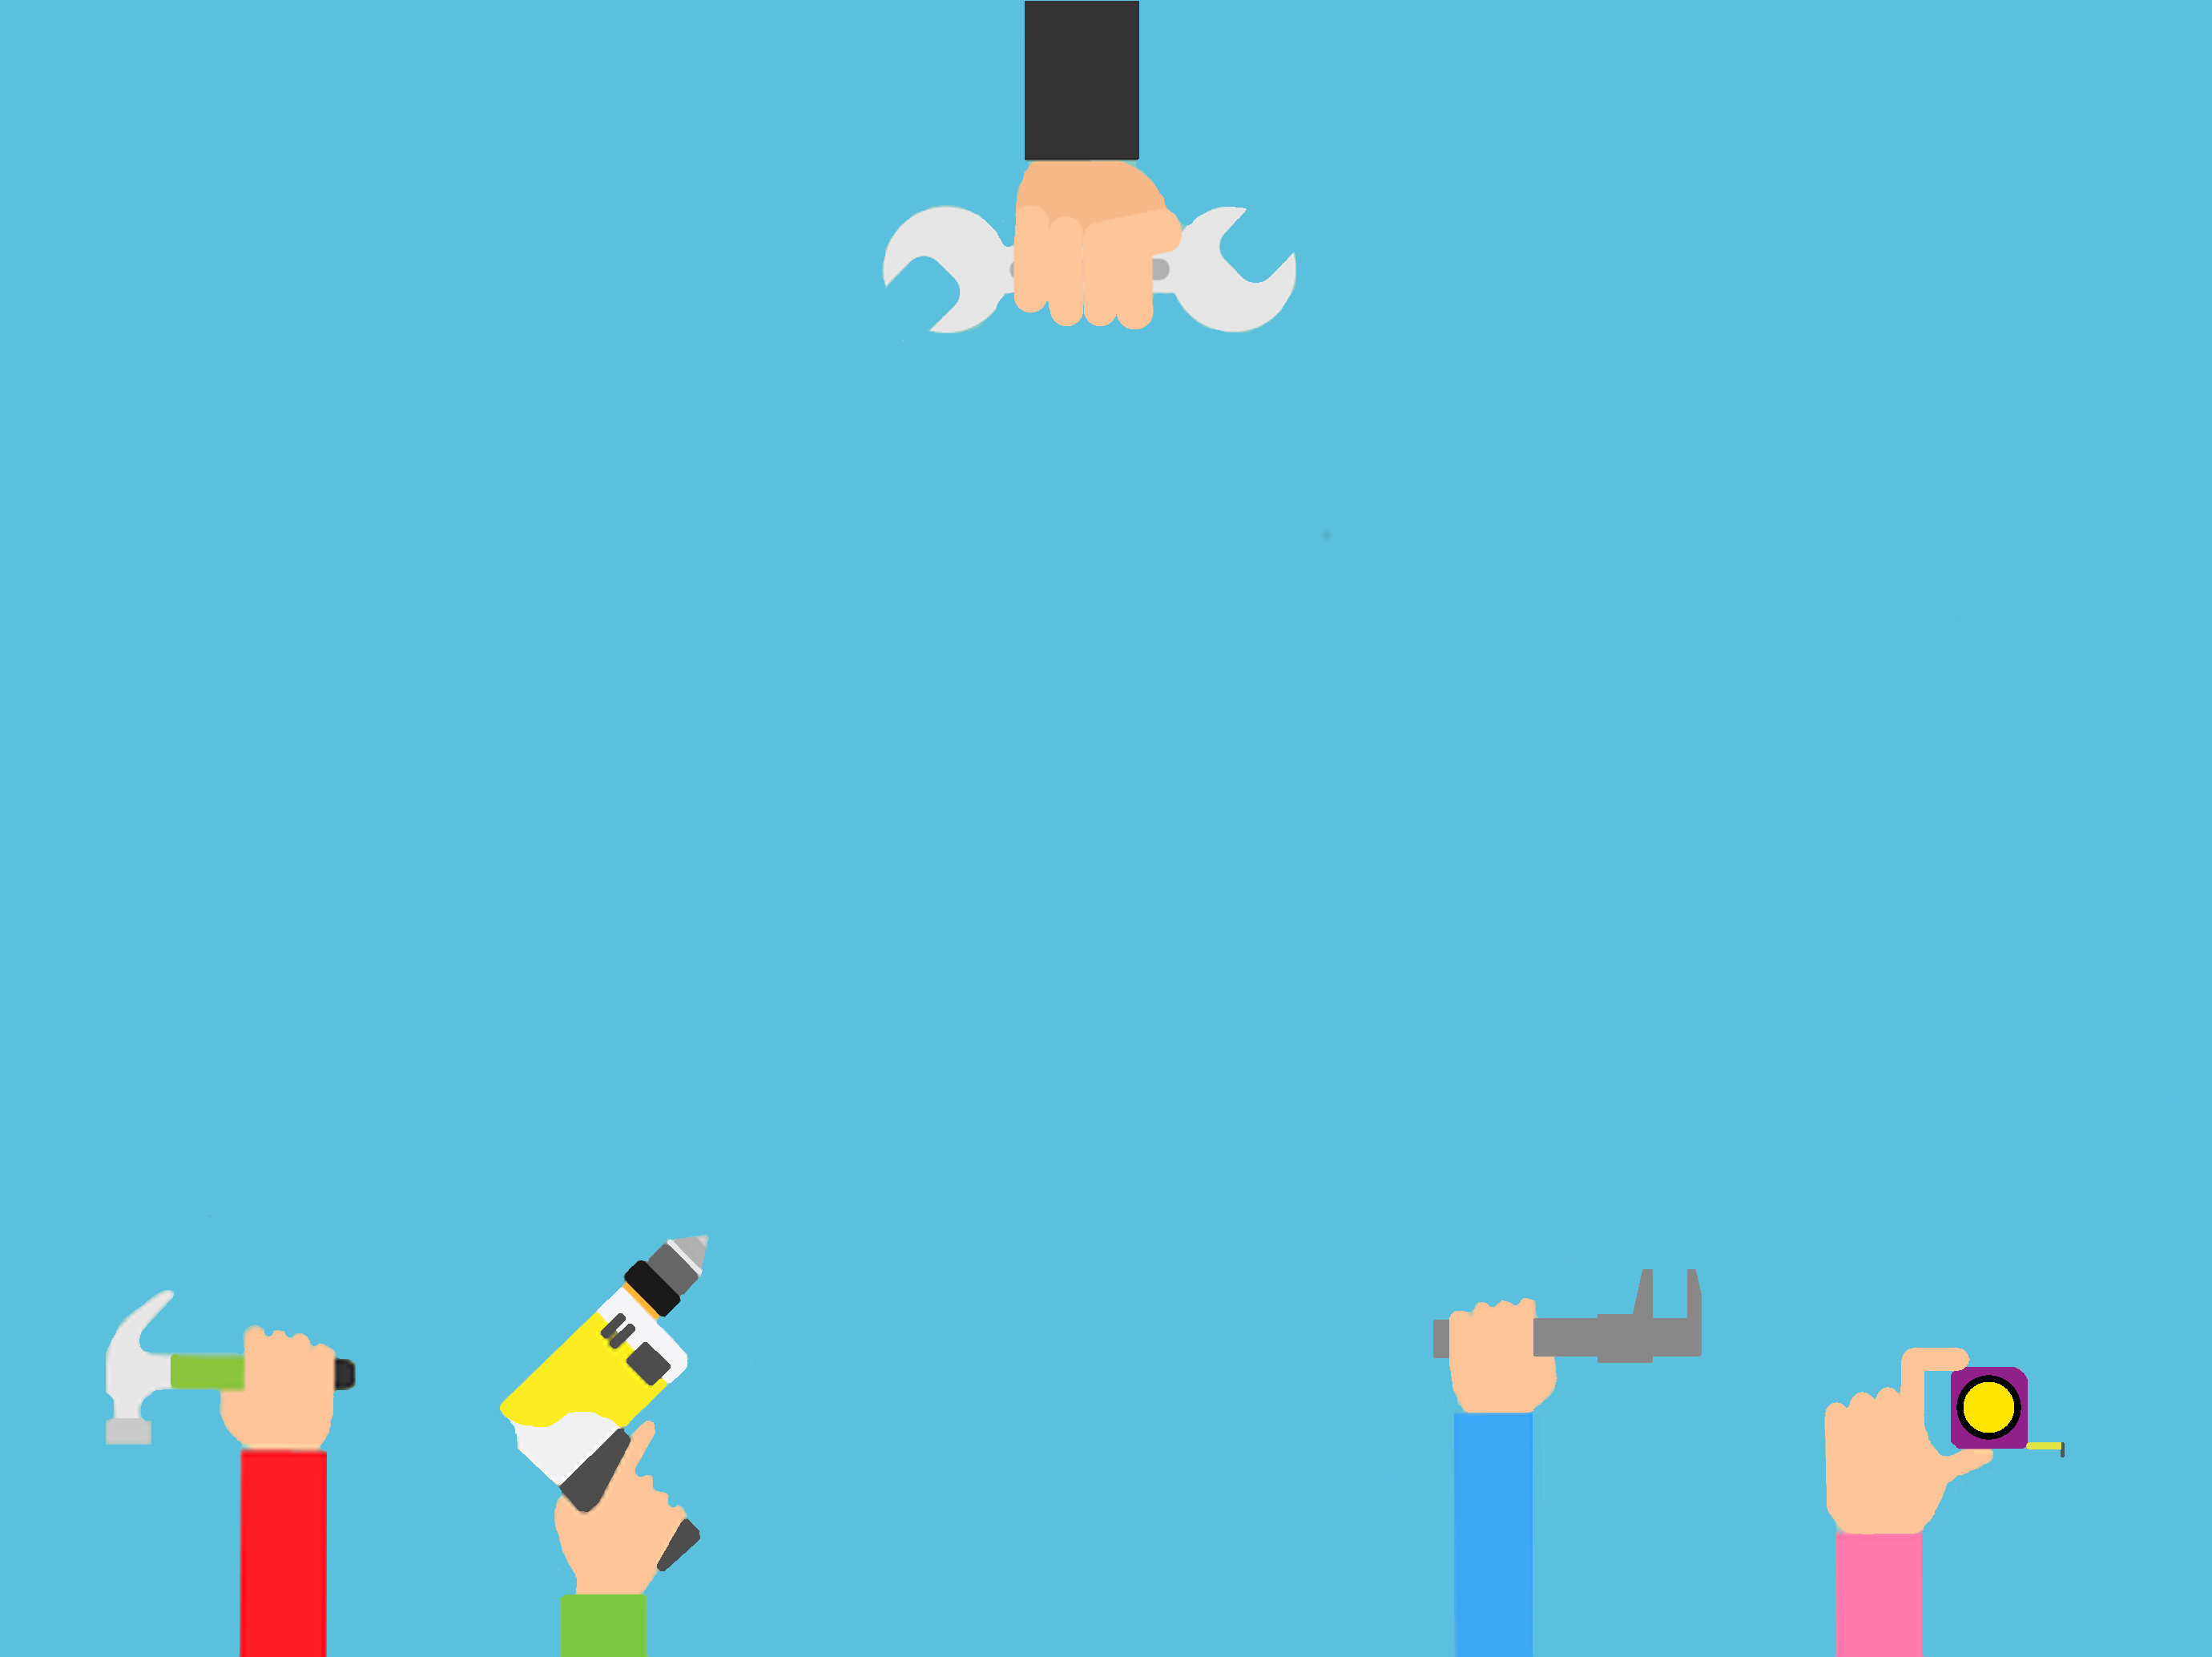
\includegraphics[width=\paperwidth]{../../img/fond}}
\frame{\titlepage}
}



\section{Introduction}

{\frame{
\frametitle{Introduction}

\begin{savoir}
Vous êtes capables :
\begin{itemize}
 \item de modéliser le comportement cinématique d'un système.
\end{itemize}
\end{savoir}

\begin{prob}
Vous devez êtes capables :
\begin{itemize}
 \item de modéliser une actions mécaniques,
 \item de déterminer comment ces actions se propagent par les pièces d'un système.
\end{itemize}
\end{prob}
}}

{\frame{
\frametitle{Modélisation vectorielle}

Une \textbf{action mécaniques} peut être considérée comme un ensemble de forces s'exerçant entre des solides. Chacune de ces forces est modélisable par un vecteur.

\vfill

\begin{minipage}{0.52\linewidth}
\begin{itemize}
 \item La force exercée sur le solide $S_1$ par $S_0$ au point A est notée $\overrightarrow{A_{S_1\rightarrow S_0}}$:
  \begin{itemize}
   \item l'\textbf{origine} du vecteur est le point du solide où s'applique la force,
   \item le \textbf{sens} et la direction du vecteur correspondent au sens et à la direction de la force,
   \item la \textbf{norme} du vecteur correspond à l'intensité, en Newton (N), de la force. 
  \end{itemize}
\end{itemize}
\end{minipage}
\hfill
\begin{minipage}{0.4\linewidth}
 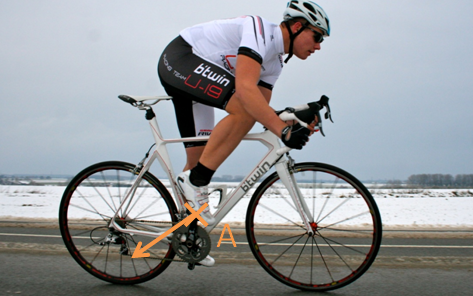
\includegraphics[width=\linewidth]{img/Diapositive1}
\end{minipage}
}}

{\frame{
\frametitle{Modélisation locale}

Il existe deux sortes d'actions mécaniques les actions à \textbf{distance} et  les actions de \textbf{contact}.

Une action mécanique d'un solide 1 sur un solide 2 est dite à \textbf{distance} si elle ne résulte pas d'une liaison mécanique entre 1 et 2. Exemple: actions magnétiques et l'action de la pesanteur.

\begin{minipage}{0.6\linewidth}
Ex: Action mécanique de pesanteur 

\begin{itemize}
 \item $\overrightarrow{df_v}=\rho.\overrightarrow{g}.dv$,
 \item $\rho$ est la masse volumique de la particule ($Kg/m^3$),
 \item $\overrightarrow{g}$ le vecteur accélération de la pesanteur ($m/s^2$), 
 \item $dV$ un élément de volume élémentaire ($m^3$). 
\end{itemize}
\end{minipage}
\hfill
\begin{minipage}{0.34\linewidth}
 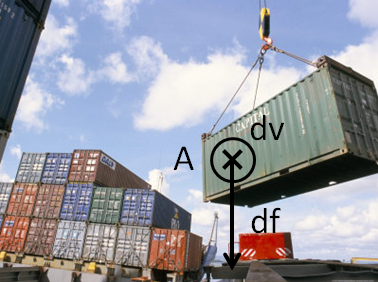
\includegraphics[width=0.8\linewidth]{img/Diapositive2}
\end{minipage}

\begin{minipage}{0.34\linewidth}
 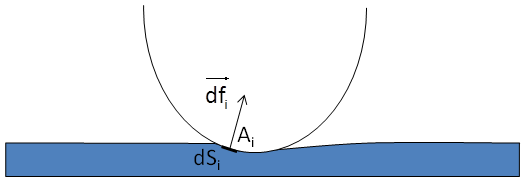
\includegraphics[width=\linewidth]{img/Diapositive3}
\end{minipage}
\hfill
\begin{minipage}{0.6\linewidth}
Ex: Pression de contact, un élément de force surfacique est donné par :

\begin{itemize}
 \item $\overrightarrow{df_s}=P.\overrightarrow{n}.ds$,
 \item $P$ est la pression de contact ($Pa$),
 \item $ds$ un élément de surface élémentaire ($m^2$), 
 \item $\overrightarrow{n}$ la normale extérieure au plan de contact.
\end{itemize}
\end{minipage}
}}


{\frame{
\frametitle{Modélisation globale d'une action mécanique}

\begin{itemize}
 \item Il est possible d'introduire le torseur, noté $\left\{ T_{\overline{S}\rightarrow S} \right\}$ qui représente l'action mécanique de $\overline{S}$ sur $S$ au point A,
 \item Le principe est donc de sommer l'ensemble des actions mécaniques
élémentaires de contact.
\end{itemize}

Étude d'un cas simplifié, nécessité du moment: $S$ subit 2 actions mécaniques élémentaires $\overrightarrow{df_1}$ et $\overrightarrow{df_2}$ aux points $A_1$ et $A_2$. Ces deux actions mécaniques élémentaires sont opposées : $\overrightarrow{df_1}=-\overrightarrow{df_2}$.

\begin{minipage}{0.7\linewidth}
\begin{itemize}
 \item Cas 1: $A_1$ est confondu avec $A_2$, $\Sigma \overrightarrow{df_i}=0$
L'action mécanique résultante de $S_0$ sur $S_0$ est nulle.
\end{itemize}
\end{minipage}
\hfill
\begin{minipage}{0.25\linewidth}
 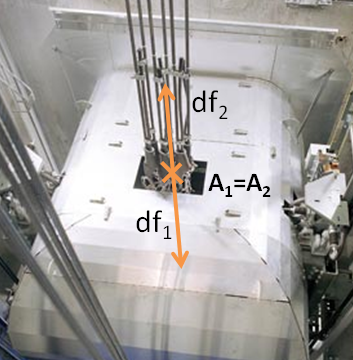
\includegraphics[width=\linewidth]{img/Diapositive4}
\end{minipage}

}}

{\frame{
\frametitle{Modélisation globale d'une action mécanique}

Étude d'un cas simplifié, nécessité du moment: $S$ subit 2 actions mécaniques élémentaires $\overrightarrow{df_1}$ et $\overrightarrow{df_2}$ aux points $A_1$ et $A_2$. Ces deux actions mécaniques élémentaires sont opposées : $\overrightarrow{df_1}=-\overrightarrow{df_2}$.

~\ \\

\begin{minipage}{0.7\linewidth}
\begin{itemize}
 \item Cas 2: $A_1$ n'est pas confondu avec $A_2$, $\Sigma \overrightarrow{df_i}=0$. L'action mécanique résultante de $\overline{S}$ sur $S$ n'est pas nulle puisque le solide $S$ est susceptible de subir une rotation sous l'effet de ces deux actions mécaniques élémentaires, donc: il faut tenir compte de la position des $A_i$ pour élaborer une action mécanique globale représentant les actions élémentaires.
\end{itemize}
\end{minipage}
\hfill
\begin{minipage}{0.25\linewidth}
 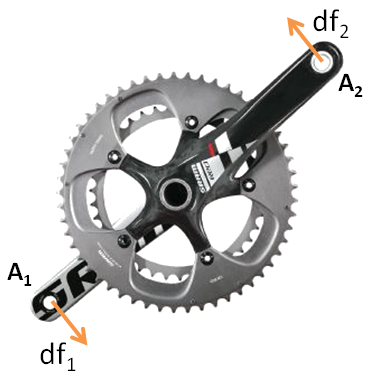
\includegraphics[width=\linewidth]{img/Diapositive5}
\end{minipage}
}}

{\frame{
\frametitle{Généralisation}

Si les actions mécaniques locales $\overrightarrow{df_{S_{Ai}}}$ (surfaciques) et $\overrightarrow{df_{V_{A_i}}}$ (volumiques) de $\overline{S}$ sur $S$ sont réparties sur les points $A_i$, on peut définir les éléments de réduction du torseur d'action mécanique de $\overline{S}$ sur $S$ de la façon suivante : 

\begin{center}
$\left\{T_{\overline{S} \rightarrow S}\right\}=\left\{\begin{array}{c}
\overrightarrow{R_{\overline{S} \rightarrow S}}=\iiint \overrightarrow{df_{V_{A_i}}} + \iint \overrightarrow{df_{S_{Ai}}} \\
\overrightarrow{M_{O,\overline{S} \rightarrow S}}=\iiint \overrightarrow{OA_i}\wedge \overrightarrow{df_{V_{A_i}}} + \iint \overrightarrow{OA_i} \wedge \overrightarrow{df_{S_{Ai}}}
\end{array}\right\}_O$
\end{center}

Remarque: Même si ce calcul intégral est rarement entrepris, il est important de comprendre ce que représente un torseur d'efforts. 
Ce torseur peut être écrit en faisant apparaitre ses composantes en projection dans un repère $R$ :

\begin{center}
$\left\{T_{\overline{S} \rightarrow S}\right\}=\left\{\begin{array}{c c}
X_{\overline{S} \rightarrow S} & L_{O,\overline{S} \rightarrow S} \\
Y_{\overline{S} \rightarrow S} & M_{O,\overline{S} \rightarrow S} \\
Z_{\overline{S} \rightarrow S} & N_{O,\overline{S} \rightarrow S}
\end{array}\right\}_O$
\end{center}
}}

{\frame{
\frametitle{Résolution analytique}

\begin{defi}
Un objet est à l'équilibre lorsqu'il a un mouvement rectiligne uniforme (son accélération linéaire et son accélération angulaire sont nulles). \\
De plus, la somme des forces et la somme des moments des forces au même point exercées sur lui sont nulles :
\begin{itemize}
 \item théorème de la résultante statique : $\sum\limits_{i=1}^n \vec{\mathrm{F}}_i = \vec{0}$,
 \item théorème du moment statique : $\sum\limits_{i=1}^n \vec{\mathrm{M}}_{\mathrm{A}}(\vec{\mathrm{F}}_i) + \sum\limits_{i=1}^n \vec{\mathrm{C}}_i = \vec{0}$.
\end{itemize}
\end{defi}

La résolution analytique avec le Principe Fondamental de la Statique se déroule en suivant la séquence suivant:
\begin{enumerate}
 \item Isoler un solide,
 \item Faire le bilan des actions mécaniques associées (de contact et à distance),
 \item Modéliser ces actions mécaniques sous la forme de torseurs,
 \item Déplacer tous ces torseurs au même point,
 \item Écrire le système d'équations issu du P.F.S.
\end{enumerate}
}}

{\frame{
\frametitle{Résolution graphique}

Dans le cas d'un problème plan ou tous les efforts sont modélisables par des glisseurs (moment nul), on peut utiliser une méthode graphique de résolution.

\begin{minipage}{0.7\linewidth}
Système soumis à 2 glisseurs coplanaires.

Soit un solide $S$ soumis en A et B à 2 glisseurs $\overrightarrow{A_{S_1 \rightarrow S}}$ et $\overrightarrow{B_{S_1 \rightarrow S}}$, par application du théorème de la résultante statique:
\begin{center}
$\overrightarrow{A_{S_1 \rightarrow S}}+\overrightarrow{B_{S_1 \rightarrow S}}=\overrightarrow{0}$, donc $\overrightarrow{A_{S_1 \rightarrow S}}=-\overrightarrow{B_{S_1 \rightarrow S}}$
\end{center}
 
Ces 2 vecteurs sont donc égaux en norme et de sens opposés, par application du théorème du moment statique en A, on a : 
\begin{center}
$\overrightarrow{AA} \wedge \overrightarrow{A_{S_1 \rightarrow S}}+\overrightarrow{AB} \wedge \overrightarrow{B_{S_1 \rightarrow S}}=\overrightarrow{0}$, donc $\overrightarrow{AB} \wedge \overrightarrow{B_{S_1 \rightarrow S}}=\overrightarrow{0}$
\end{center}

$\overrightarrow{B_{S_1 \rightarrow S}}$ est donc colinéaire à $\overrightarrow{AB}$. Donc $\overrightarrow{A_{S_1 \rightarrow S}}$ aussi. 

~\ \\

Les 2 glisseurs ont le même support, \textbf{la droite passant par les 2 points d'application}, ils sont de même norme et de sens opposés.

\end{minipage}\hfill
\begin{minipage}{0.25\linewidth}
 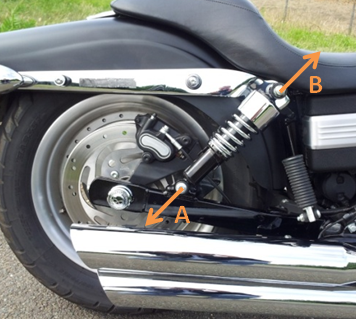
\includegraphics[width=\linewidth]{img/Diapositive6} \\
 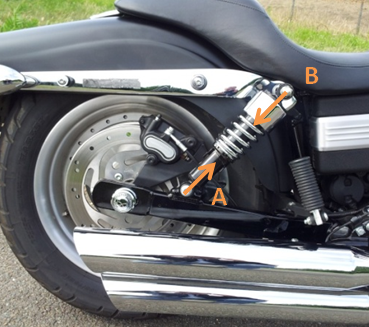
\includegraphics[width=\linewidth]{img/Diapositive7}
\end{minipage}

}}


{\frame{
\frametitle{Résolution graphique}

\begin{minipage}{0.7\linewidth}
Système soumis à 2 glisseurs coplanaires.\\
Soit un solide $S$ soumis en A, B et C à 3 glisseurs $\overrightarrow{A_{S_1 \rightarrow S}}$, $\overrightarrow{B_{S_1 \rightarrow S}}$ et $\overrightarrow{C_{S_1 \rightarrow S}}$, par application du théorème de la résultante statique, on a : $\overrightarrow{A_{S_1 \rightarrow S}}+\overrightarrow{B_{S_1 \rightarrow S}}+\overrightarrow{C_{S_1 \rightarrow S}}=\overrightarrow{0}$

Cette somme vectorielle nulle peut être traitée de façon graphique en construisant un triangle appelé le triangle le dynamique fermé. 

Par application du théorème du moment statique en I, on a : 

$\overrightarrow{IA} \wedge \overrightarrow{A_{S_1 \rightarrow S}}+\overrightarrow{IB} \wedge \overrightarrow{B_{S_1 \rightarrow S}}+\overrightarrow{IC} \wedge \overrightarrow{C_{S_1 \rightarrow S}}=\overrightarrow{0}$

Soit I à l'intersection des supports de $\overrightarrow{A_{S_1 \rightarrow S}}$ et $\overrightarrow{B_{S_1 \rightarrow S}}$,

$\overrightarrow{IA} \wedge \overrightarrow{A_{S_1 \rightarrow S}}=\overrightarrow{IB} \wedge \overrightarrow{B_{S_1 \rightarrow S}}=\overrightarrow{0}$.

Ainsi, $\overrightarrow{IC} \wedge \overrightarrow{C_{S_1 \rightarrow S}}=\overrightarrow{0}$, donc I appartient également à la direction de $\overrightarrow{C_{S_1 \rightarrow S}}$.

Les trois glisseurs sont donc concourants en I, leur somme vectorielle est nulle.

\end{minipage}\hfill
\begin{minipage}{0.25\linewidth}
 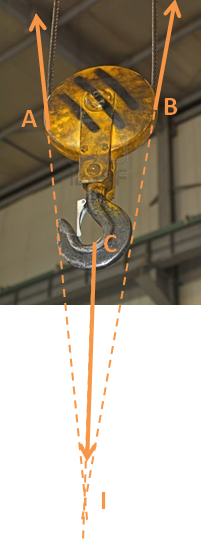
\includegraphics[width=0.9\linewidth]{img/Diapositive9}
\end{minipage}
}}

{\frame{
\frametitle{Conclusion}

\begin{savoir}
Vous êtes capables :
\begin{itemize}
 \item de modéliser une action mécanique,
 \item résoudre un problème de statique en utilisant le P.F.S.
\end{itemize}
\end{savoir}

\begin{prob}
Vous devez êtes capables de :
 \begin{itemize}
  \item modéliser les actions de contact avec frottements.
 \end{itemize} 
\end{prob}
}}

\end{document}